\documentclass[tikz]{standalone}
\usepackage{tikz}
\usetikzlibrary{
	shapes,
	snakes,
	calc,
	decorations,
	decorations.markings,
	decorations.text,
	decorations.pathreplacing}
	
\begin{document}
	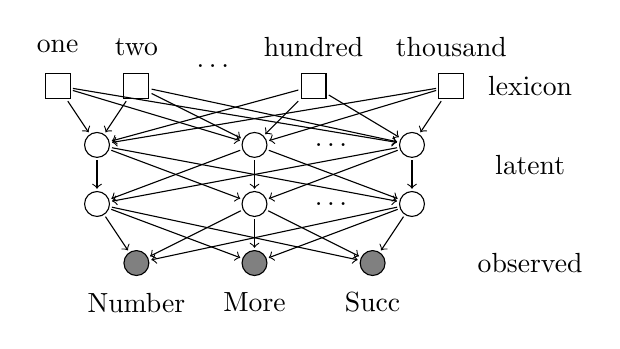
\begin{tikzpicture}[scale=1,every text node part/.style={align=left}]
		\tikzstyle{vertex}=[circle,draw,minimum size=9pt,
                  inner sep=1pt, outer sep=1pt]
		\tikzstyle{vbox}=[rectangle,draw,minimum size=9pt,
                  inner sep=1pt, outer sep=1pt]
    	
     	\foreach \name/\x in {Number/.5, More/2, Succ/3.5}
       		\node[] (\name) at (\x,.5) {\name};


     	\foreach \name/\x in {one/-.5, two/.5, hundred/2.75, thousand/4.5}
       		\node[] (\name) at (\x,3.75) {\name};
    	\node (Adots2) at (1.5 ,3.5) {\ldots};

     	\foreach \name/\x in {W/-.5, X/.5, Y/2.75, Z/4.5}
       		\node[vbox] (\name) at (\x,3.25) {};

        
    	\foreach \name/\x in {A/0, B/2, C/4}
       		\node[vertex] (\name) at (\x,1.75) {};
    	\node (Adots2) at (3 ,1.75) {\ldots};

    	\foreach \name/\x in {D/0, E/2, F/4}
       		\node[vertex] (\name) at (\x,2.5) {};
    	        \node (Adots2) at (3 ,2.5) {\ldots};

    	\foreach \name/\x in {G/.5, H/2, I/3.5}
       		\node[vertex,fill=black!50] (\name) at (\x,1) {};

        % edges

        \foreach \wname in {A, B, C}
            \foreach \aname in {D, E, F}
                \draw [<-] (\wname) -- (\aname);

        \foreach \wname in {W, X, Y, Z}
            \foreach \aname in {D, E, F}
                \draw [->] (\wname) -- (\aname);

        \foreach \wname in {A, B, C}
            \foreach \aname in {G, H, I}
                \draw [->] (\wname) -- (\aname);

        \node (lex) at (5.5,3.25) {lexicon};
        \node (lat) at (5.5,2.25) {latent};
        \node (obs) at (5.5,1) {observed};
                

	\end{tikzpicture}
\end{document}

%%% Local Variables:
%%% mode: latex
%%% TeX-master: t
%%% End:
